\documentclass[aspectratio=1610]{beamer}

\usetheme{KTH}
\useinnertheme[shadow]{rounded}
\setbeamercolor{block title example}{fg=black,bg=lightgray}
\setbeamercolor{block body example}{fg=white,bg=gray}
\setbeamercolor{block body}{fg=white,bg=blue!60}

% remove this if using XeLaTeX or LuaLaTeX
\usepackage[utf8]{inputenc}
\usepackage{graphics}
\usepackage{graphicx}
\usepackage{booktabs}
\usepackage{ragged2e}
\usepackage{lipsum}
\usepackage{minted}
\usepackage{tikz}
\usepackage{array}
\usepackage{algorithm,algorithmicx}
\usepackage{algpseudocode}
\usepackage{amsmath,amsfonts,amssymb}
\usepackage[export]{adjustbox}
\setbeamertemplate{caption}[numbered]
\usepackage{bbding}
\usepackage{siunitx}

\setbeamercolor{itemize item}{fg=darkred}
\setbeamercolor{itemize subitem}{fg=TextGreen}
\setbeamercolor{itemize subbody}{fg=LightGray}
\newcommand{\norm}[1]{\left\lVert#1\right\rVert}

\setbeamertemplate{itemize item}{\scriptsize\raise1.25pt\hbox{\donotcoloroutermaths$\blacktriangleright$}}
\setbeamertemplate{itemize subitem}{\tiny\raise1.5pt\hbox{\donotcoloroutermaths$\bullet$}}
\setbeamertemplate{itemize subsubitem}{\tiny\raise1.5pt\hbox{\donotcoloroutermaths$\blacksquare$}}


\begin{document}

%------------------------------------------------
\begin{frame}[noframenumbering,plain]

  \vspace{0.02\textheight}

\begin{columns}[]
\column{37em}
\Large{\centerline{\usebeamercolor[fg]{title}Estimation of the Mass of a Manipulator Payload in Motion}}

\Large{\centerline{\usebeamercolor[fg]{title} by Means of a FT Sensor}}

\vspace{0.1\textheight}

\small{\centerline{François \textsc{Le Rall}}}
\scriptsize{\centerline{\tt flr@kth.se}}
\scriptsize{\centerline{}}
\end{columns}
\end{frame}

%------------------------------------------------
\usebackgroundtemplate{\vbox{\null\vspace{3mm}
  \hspace{3mm}\pgfuseimage{kthlogosmall}\par
  \vspace{72mm}\hbox{\hspace{-75mm}\pgfuseimage{kthplatta}}}}

%------------------------------------------------
\begin{frame}
\frametitle{\textit{Pick-and-place} at its very beginning}

\begin{figure}
\centering
  \begin{minipage}{.49\textwidth}
  \centering
  \includegraphics[width=.9\linewidth]{figs/kid.jpg}
  \caption{Kid experiencing \textit{P\&P}}
  \end{minipage}
  \begin{minipage}{.49\textwidth}
  \centering
  \includegraphics[width=.9\linewidth]{figs/unimation.jpg}
  \caption{\footnotesize \textsc{Unimate}: first \textit{P\&P} robot (1954)}
  \end{minipage}
\end{figure}
\end{frame}

%------------------------------------------------
\begin{frame}
\frametitle{Automation of industrial tasks}
\begin{columns}
\begin{column}{0.5\textwidth}
  \begin{itemize}\itemsep1em
    \justifying
    \item \textcolor{Ocean}{Fulfill} customer's orders
    \item \textcolor{Ocean}{Place} electronic components on Printed Circuit Board
    \item \textcolor{Ocean}{Assemble} products (automotive, electronic)
    \item \textcolor{Ocean}{Load} and \textcolor{Ocean}{unload} manufacturing systems
  \end{itemize}
\end{column}
\begin{column}{0.5\textwidth}  %%<--- here
  \begin{figure}
    \centering
    \includegraphics[width=\linewidth]{figs/maria.jpg}
    \caption{\textit{E-commerce} picking robot}
  \end{figure}
\end{column}
\end{columns}

\end{frame}

%------------------------------------------------
\begin{frame}
\frametitle{Industrial challenges}
\begin{columns}
\column{37em}
\begin{itemize}\itemsep1em
  \justifying
  \item Handle a wide \textcolor{Ocean}{diversity of objects}
  \item Pick \textcolor{Ocean}{unknown items} at \textcolor{Ocean}{unknown positions}
  \item Execute tasks \textcolor{Ocean}{faster and faster}
  \item \textcolor{Ocean}{Minimize hard failures} requiring human intervention
  \item Perform \textcolor{Ocean}{object recognition} or \textcolor{Ocean}{pose estimation} while running the \textit{P\&P} tasks
  \item \textcolor{Ocean}{Adapt trajectories} to the item handled
\end{itemize}
\end{columns}
\end{frame}

%------------------------------------------------
\begin{frame}
\frametitle{Motivations behind mass estimation}
\begin{columns}
\column{37em}
\begin{itemize}\itemsep1em
  \justifying
  \item Feature for \textcolor{Ocean}{item recognition}
  \item Parameter for highly-dynamic \textcolor{Ocean}{force-guided} or \textcolor{Ocean}{force-guarded motion}
  \item Attribute to detect \textcolor{Ocean}{hard failures}:
  \begin{itemize}\itemsep1em
    \justifying
    \item two items grasped instead of one
    \item item lost during motion
    \item item hit due to oversize
  \end{itemize}
  \item Valuable parameter for \textcolor{Ocean}{item pose estimation}
  \item Feature to detect \textcolor{Ocean}{product anomalies}
\end{itemize}
\end{columns}
\end{frame}

%------------------------------------------------
\begin{frame}
\frametitle{Hardware setup}
\begin{columns}
\begin{column}{0.5\textwidth}
  \begin{itemize}\itemsep1em
    \justifying
    \item UR10e robotic manipulator from \textsc{Universal Robot}
    \item Pneumatic \textcolor{Ocean}{vacuum gripper}
    \item Force/Torque (FT) sensor mounted on the \textcolor{Ocean}{last wrist}
    \item \textit{Pick-and-place} tasks:
    \begin{itemize}\itemsep0.0em
      \justifying
      \item tote to tote
      \item cart to box
    \end{itemize}
  \end{itemize}
\end{column}
\begin{column}{0.5\textwidth}  %%<--- here
  \begin{figure}
    \centering
    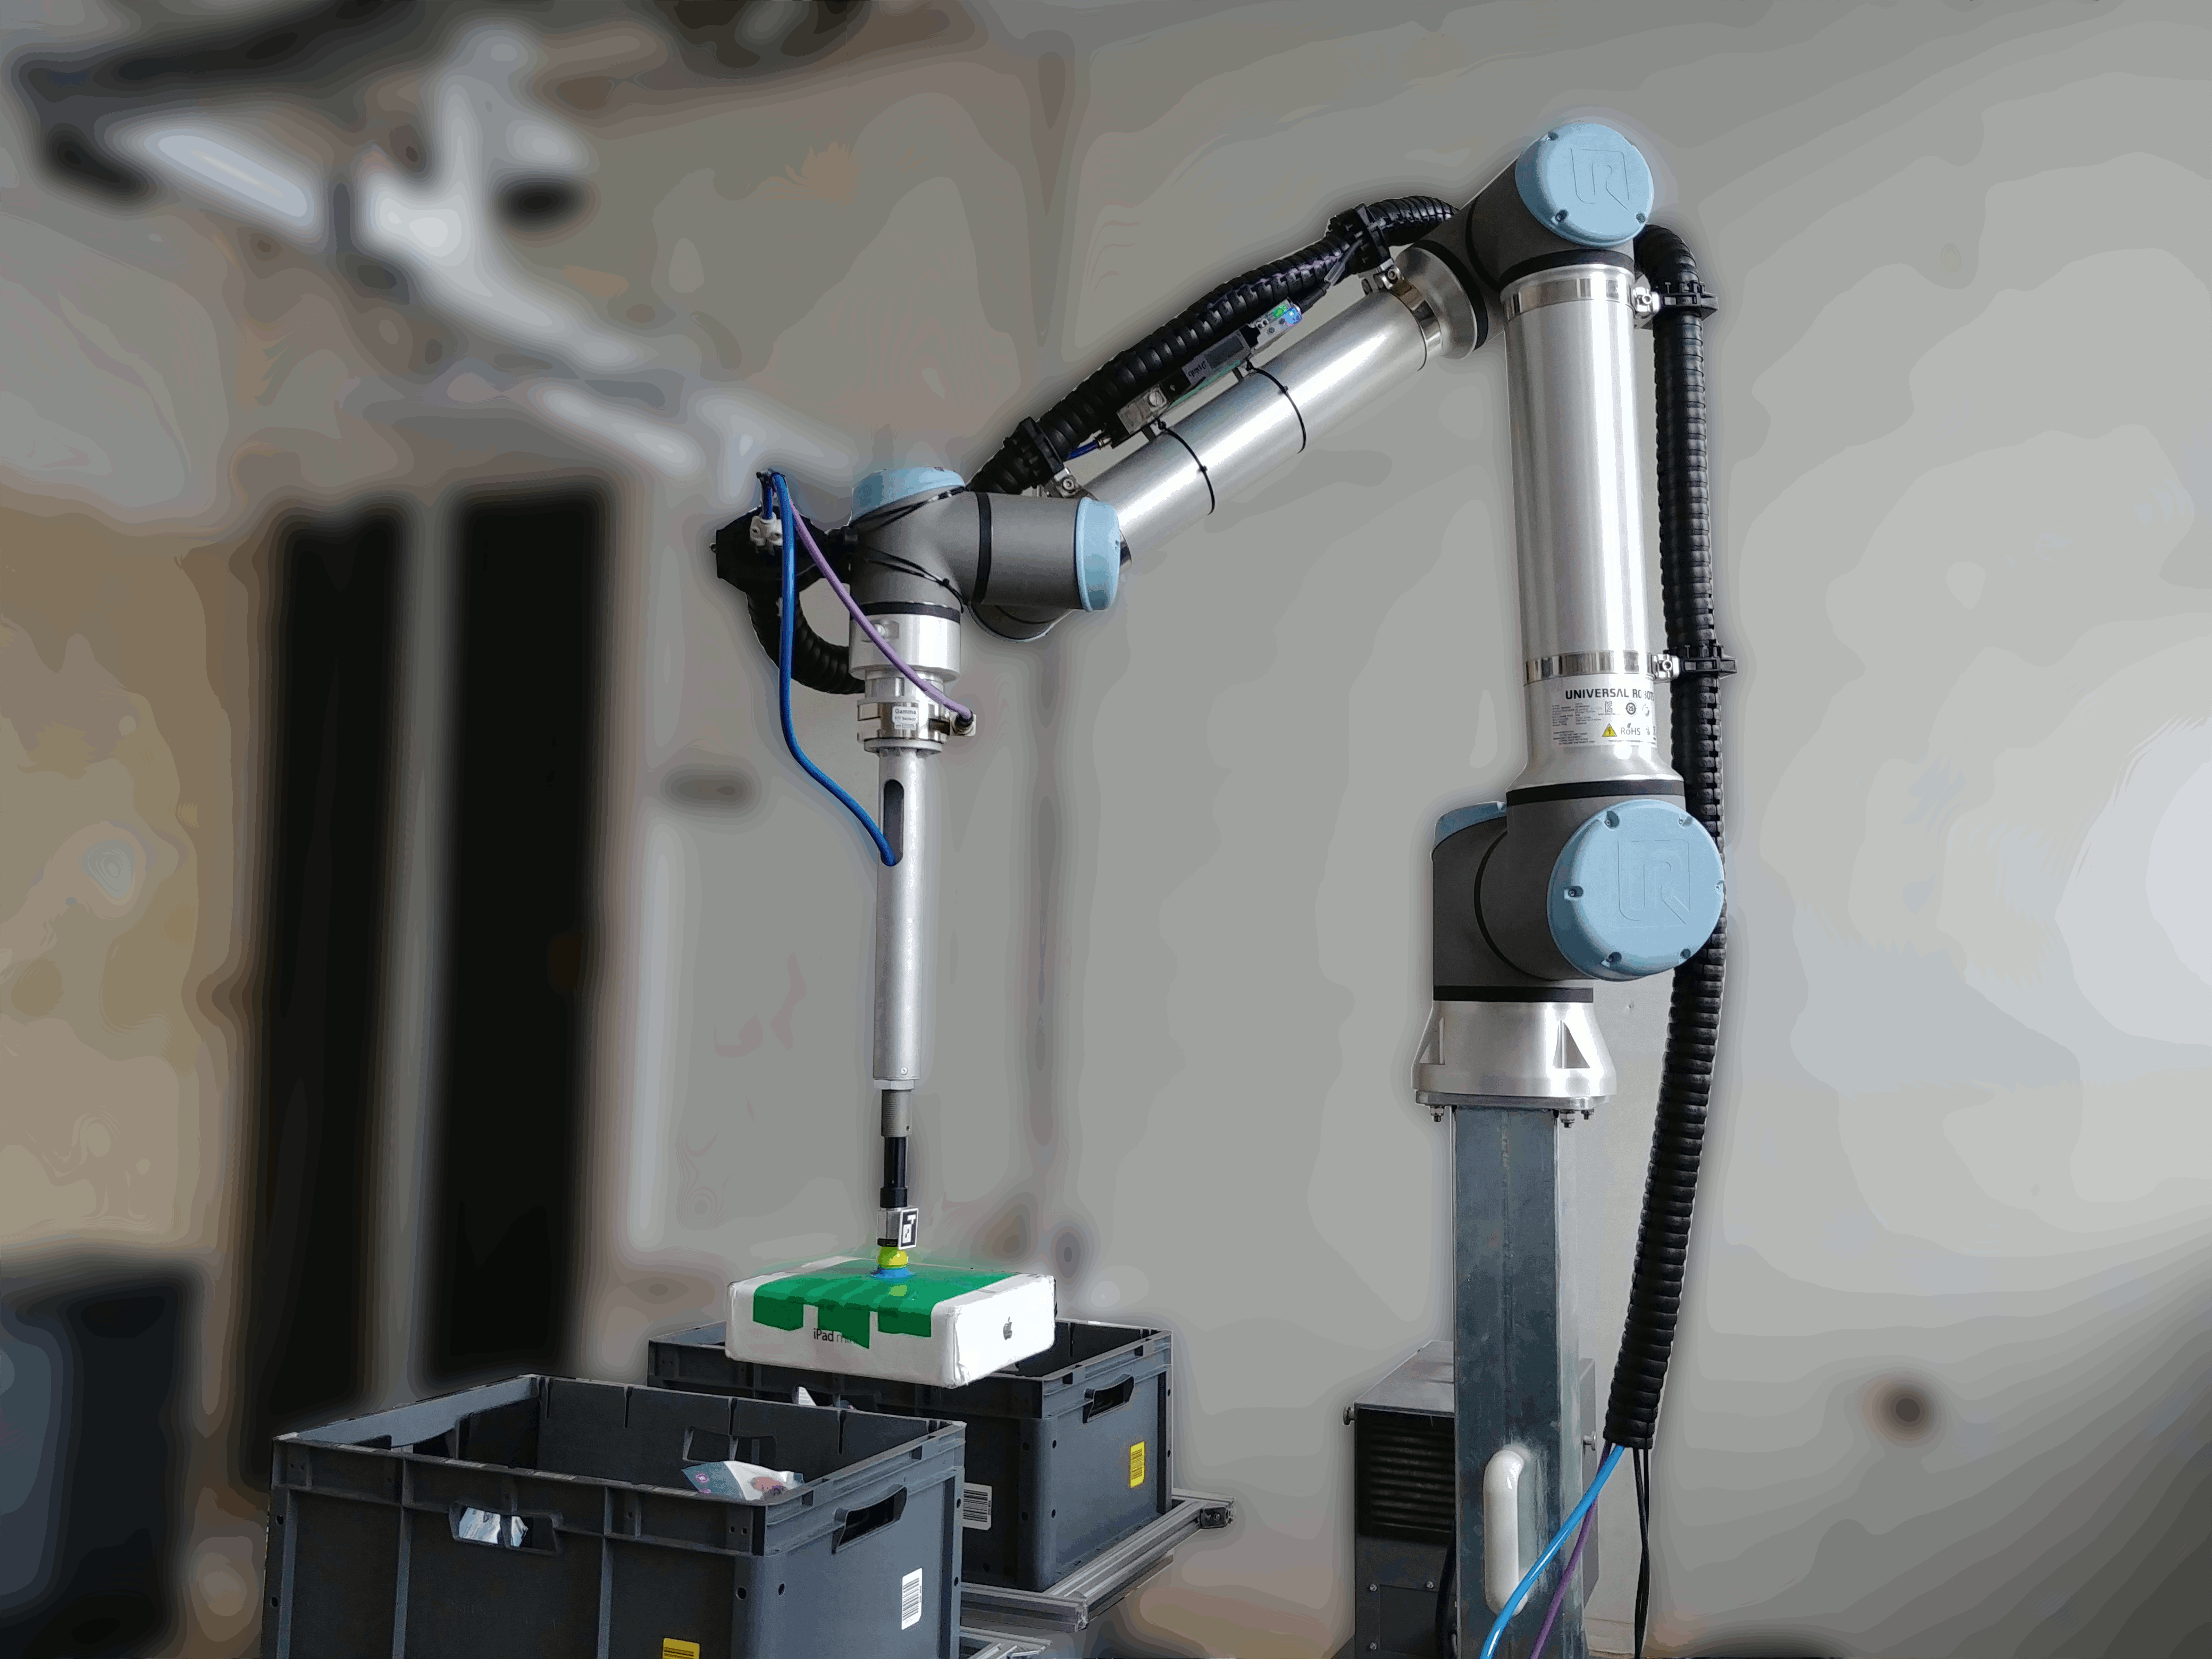
\includegraphics[width=\linewidth]{figs/picture_of_ur_indexed.png}
    \caption{UR10e robotic arm}
  \end{figure}
\end{column}
\end{columns}

\end{frame}

%------------------------------------------------
\begin{frame}
\frametitle{Suction cup gripper}
\begin{columns}
\begin{column}{0.5\textwidth}
  \begin{itemize}\itemsep1em
    \justifying
    \item \textcolor{TextGreen}{Simple integration logic}
    \item \textcolor{TextGreen}{Versatile ability to grasp objects}
    \item \textcolor{TextGreen}{Good grip on large range of textures}
    \item \textcolor{darkred}{Risk of item lost}
    \item \textcolor{darkred}{Oscillation during the motion}
    \item \textcolor{darkred}{No existing model of the mechanical link between the tool and the item}
  \end{itemize}
\end{column}
\begin{column}{0.5\textwidth}  %%<--- here
  \begin{figure}
    \centering
    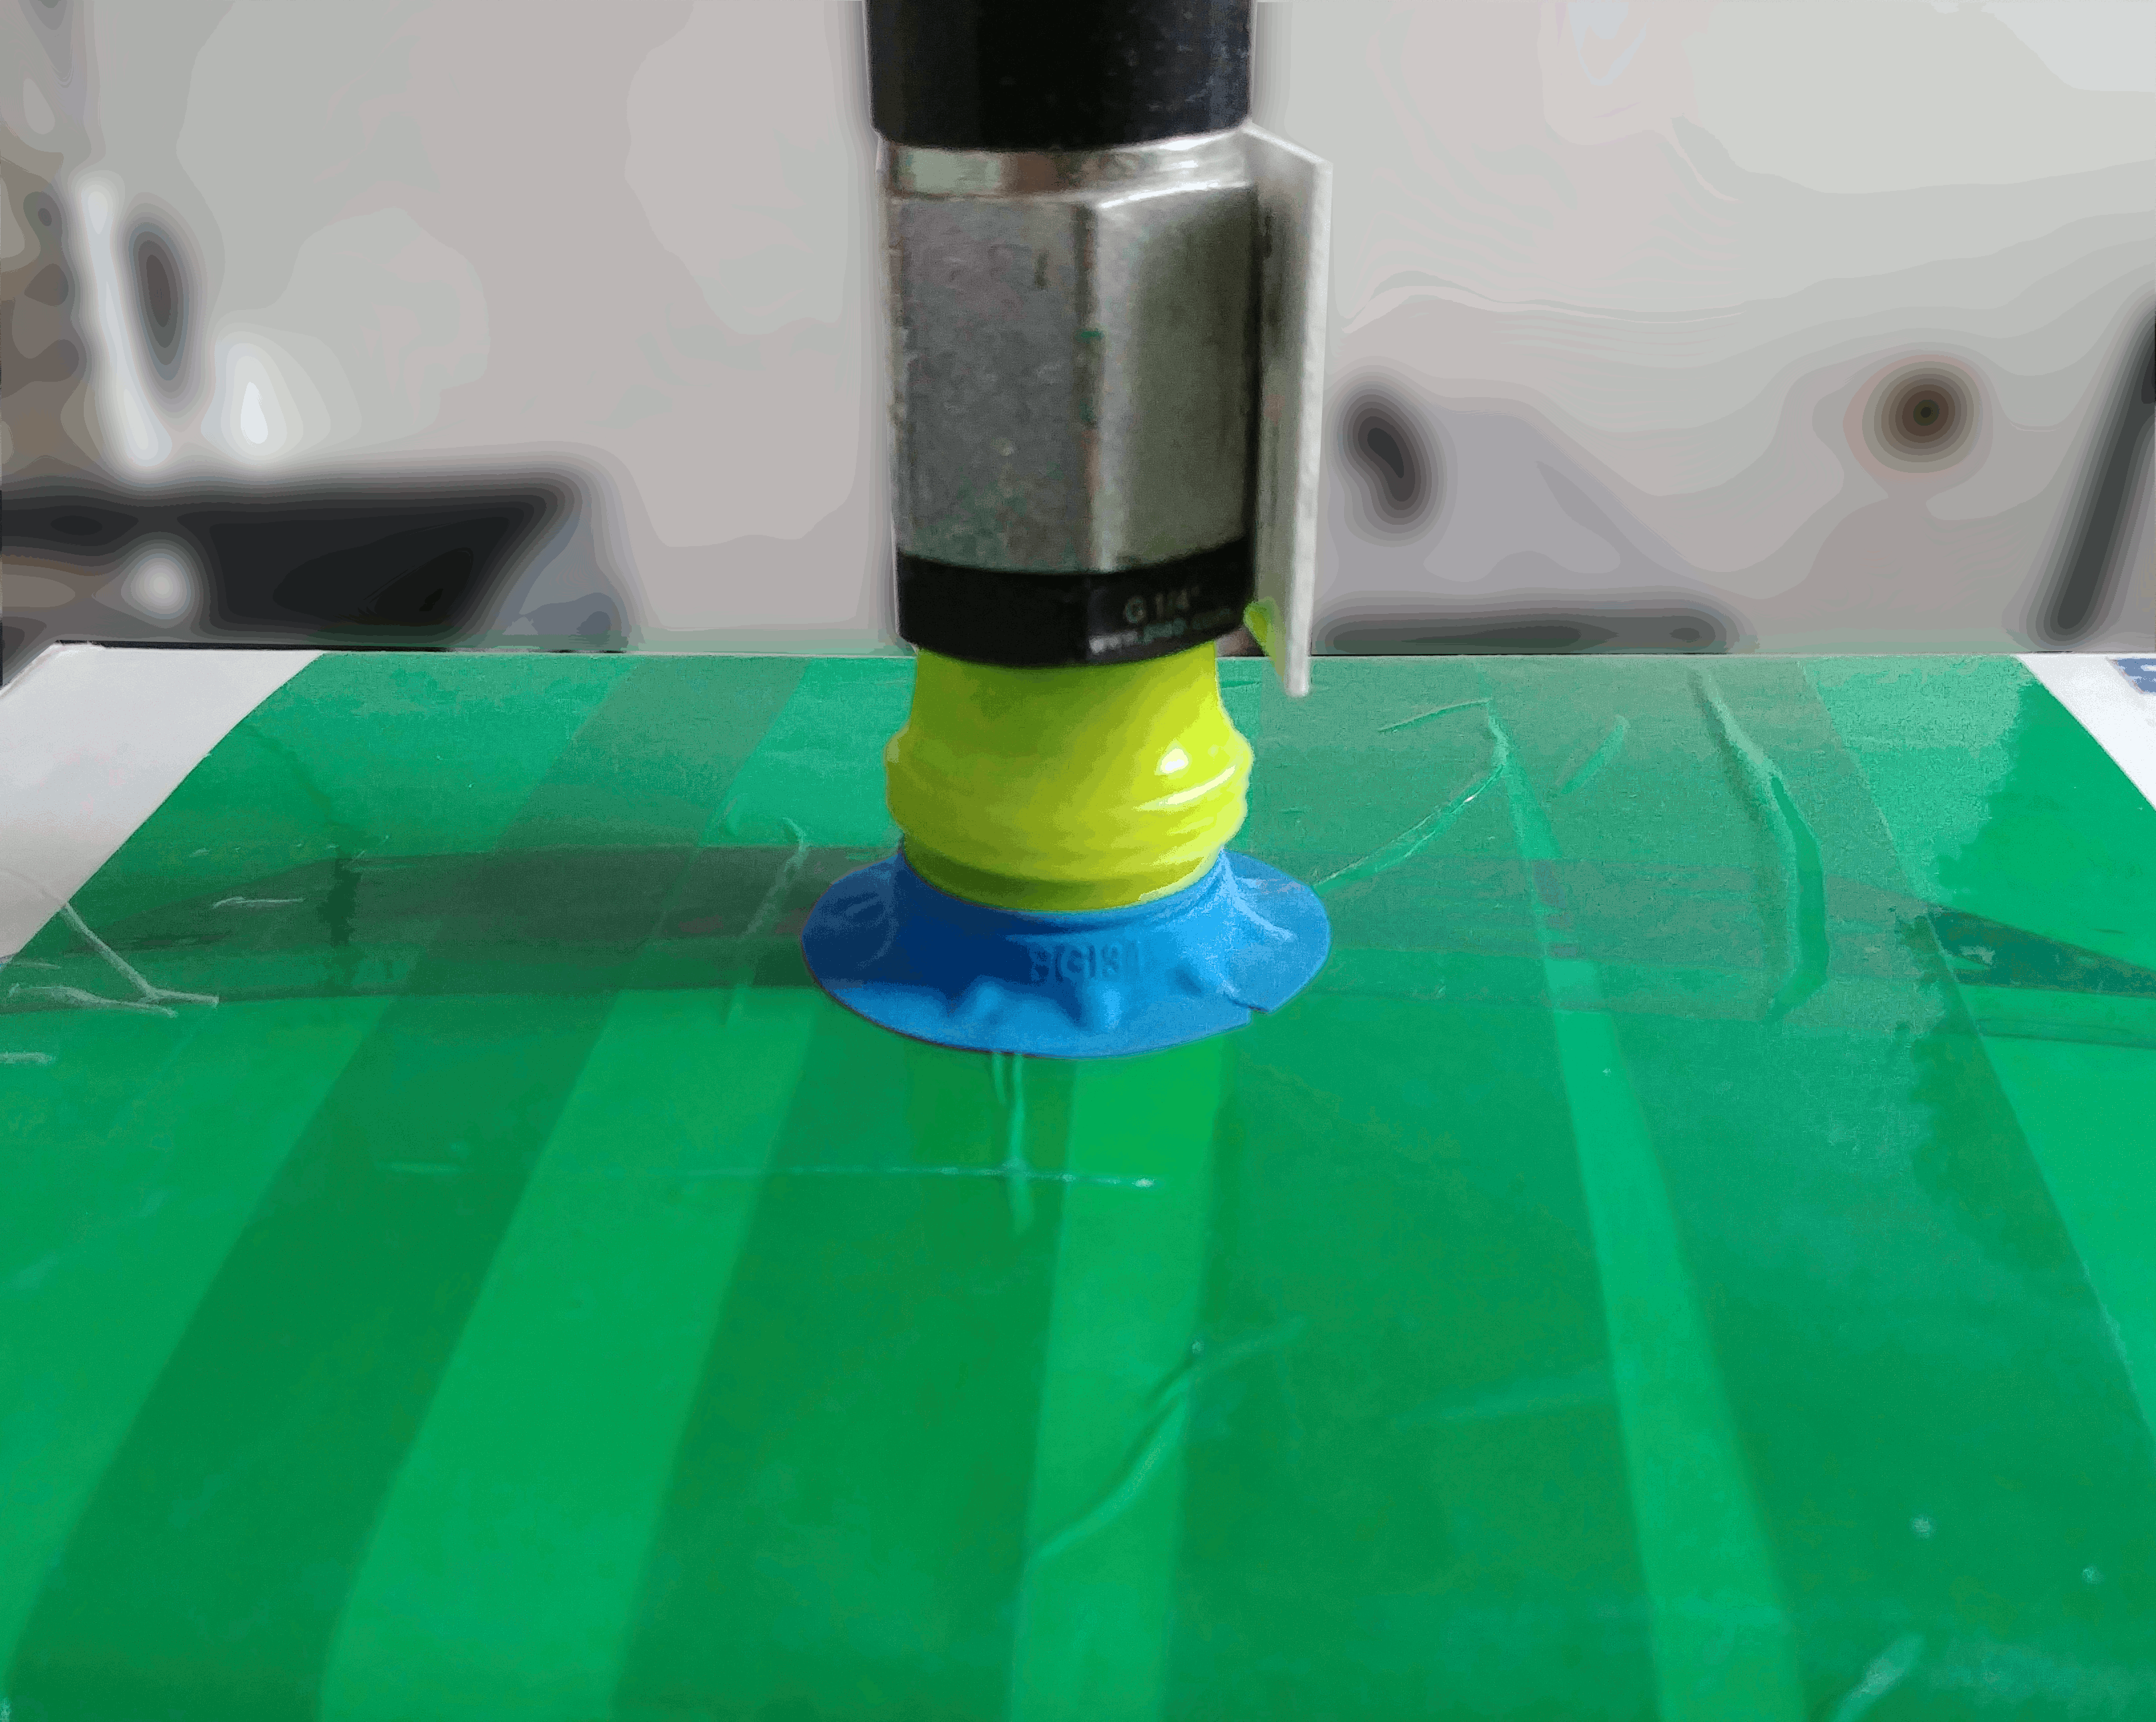
\includegraphics[scale=0.055]{figs/suction_loaded_indexed.png}
    \caption{Suction cup gripper}
  \end{figure}
\end{column}
\end{columns}

\end{frame}

%------------------------------------------------
\begin{frame}
\frametitle{Approach requirements}
\begin{columns}
\column{37em}
\begin{itemize}\itemsep1em
  \justifying
  \item Applicable to a \textcolor{Ocean}{wide range of objects} with different:
  \begin{itemize}
    \item sizes
    \item shapes
    \item masses (from $0.0 \si{\kilogram}$ to $\sim 1.0 \si{\kilogram}$)
    \item packagings (cardboard, foil)
  \end{itemize}
  \item \textcolor{Ocean}{No modification} of the trajectory of the robot necessary
  \item \textcolor{Ocean}{Online} or \textcolor{Ocean}{quick offline} mass computations
  \item Suitable to a all kind of robotic manipulators with \textcolor{Ocean}{FT sensor} and \textcolor{Ocean}{suction cup}
\end{itemize}

\end{columns}
\end{frame}

%------------------------------------------------
\begin{frame}
\frametitle{Project background – Literature review}
\begin{columns}
\column{37em}
\begin{itemize}\itemsep1em
  \justifying
  \item \textbf{\textcolor{TextGreen}{\textsc{Liu} and \textsc{An}}}: Inertial parameters of the links of the robotic manipulator
  \begin{itemize}
    \item \textcolor{Ocean}{FT sensor} mounted between the base and the first link \textcolor{darkred}{\XSolidBrush}
    \item computation of the \textcolor{Ocean}{kinematics} of every part the robot
    \item \textcolor{Ocean}{Least-Squares} optmization with \textcolor{Ocean}{\textsc{Newton-Euler} equations}
    \item \textcolor{Ocean}{excitation trajectories} \textcolor{darkred}{\XSolidBrush}
  \end{itemize}
  \item \textbf{\textcolor{TextGreen}{\textsc{Kubus} and \textsc{Farsoni}}}: Inertial parameters of the payload
  \begin{itemize}
    \item \textcolor{Ocean}{FT sensor} mounted on the last wrist \textcolor{TextGreen}{\CheckmarkBold}
    \item computation of the \textcolor{Ocean}{kinematics} of the TCP
    \item enhanced \textcolor{Ocean}{Least-Squares} optmization with \textcolor{Ocean}{\textsc{Newton-Euler} equations}
    \begin{itemize}
      \item Recursive Least-Squares
      \item \textsc{Kalman} filter
    \end{itemize}
    \item \textcolor{Ocean}{excitation trajectories} \textcolor{darkred}{\XSolidBrush}
  \end{itemize}
\end{itemize}

\end{columns}
\end{frame}

%------------------------------------------------
\begin{frame}
\frametitle{Framework for the estimation of the mass}
\begin{columns}
\column{37em}
\begin{figure}
  \centering
  \includegraphics[width=\linewidth]{figs/olinpe.pdf}
  \caption{Overview of the approach to estimate $\varphi = [ m, c_{x}, c_{y}, c_{z}, I_{xx}, I_{xy}, I_{xz}, I_{yy}, I_{yz}, I_{zz} ]$}
\end{figure}\end{columns}
\end{frame}

%------------------------------------------------
\begin{frame}
\frametitle{Rigid link mechanical model}
\begin{columns}
\begin{column}{0.5\textwidth}
  \begin{itemize}\itemsep1em
    \justifying
    \item System: \{tool (1) + item (2)\}
    \item Mechanical link: rigid – forces and torques fully transmitted
    \item Fondamental Principle of Dynamics: \\
    \vspace{0.3cm}
      $f = m (a - g) + \omega \times (\omega \times m c) + \alpha \times m c$ \\
      $\tau = m c \times (a - g)
      + I_{A} \ast \alpha + \omega \times (I_{A} \ast \omega)$
    \item Matrix form: \\
    \vspace{0.5cm}
    $\begin{pmatrix}
      f    \\
      \tau
     \end{pmatrix}
     = A(a, \alpha, \omega, g) \varphi$

  \end{itemize}
\end{column}
\begin{column}{0.5\textwidth}  %%<--- here
  \begin{figure}
    \centering
    \includegraphics[scale=0.65]{figs/one_body.pdf}
  \end{figure}
\end{column}
\end{columns}

\end{frame}

%------------------------------------------------
\begin{frame}
\frametitle{Rotational Mass Spring Damper model}
\begin{columns}
\begin{column}{0.5\textwidth}
  \begin{itemize}\itemsep1em
    \justifying
    \item Systems: \{tool (1)\} and \{item (2)\}
    \item Mechanical link: forces and torque about $z_1$-axis transmitted
    \item Rotational Spring Damper: \\
    $T_{2/1} = K \ast \overrightarrow{\Theta}_{2/1} + \Lambda \ast \overrightarrow{\Omega}_{2/1}$
    \begin{itemize}
      \item $K = diag(k, k, 0)$
      \item $\Lambda = diag(\lambda, \lambda, 0)$
    \end{itemize}
    \item Matrix form: \\
    \vspace{0.5cm}
    $\begin{pmatrix}
      f'    \\
      \tau'
     \end{pmatrix}
     = A'(a, \alpha, \omega, g) \varphi_2$

  \end{itemize}
\end{column}
\begin{column}{0.5\textwidth}  %%<--- here
  \begin{figure}
    \centering
    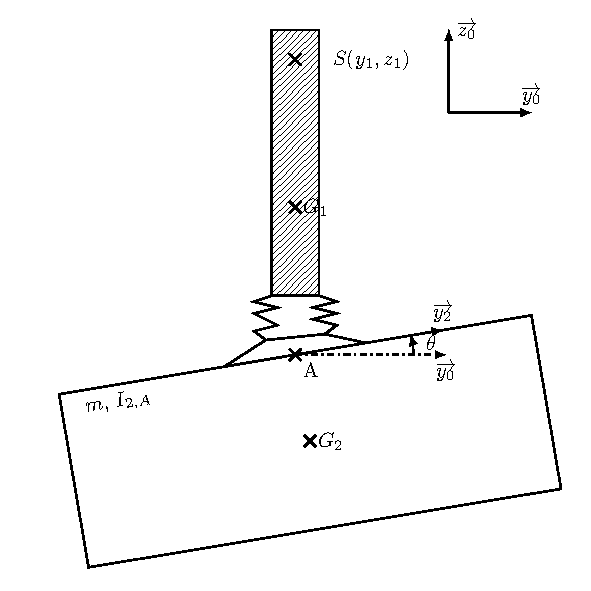
\includegraphics[scale=0.65]{figs/two_bodies.pdf}
  \end{figure}
\end{column}
\end{columns}

\end{frame}

%------------------------------------------------
\begin{frame}
\frametitle{Calibration of the properties of the system}
\begin{columns}
\column{37em}
\begin{itemize}\itemsep1em
  \justifying
  \item Inertial parameters of the tool
  \begin{itemize}
    \item End-effectors are likely to be unique creations
    \item No ground-truth values provided
    \item Estimation with the rigid model
  \end{itemize}
  \item Spring coefficient and damping coefficient of the suction cup
  \begin{itemize}
    \item As many parameters as there are suction cups
    \item Estimation with the RMSD model and a standard item:
    \begin{itemize}
      \item Mass $m_2$
      \item Center of mass $c_2$
      \item Inertia tensor $I_2$
    \end{itemize}
  \end{itemize}
\end{itemize}
\end{columns}
\end{frame}

%------------------------------------------------
\begin{frame}
\frametitle{Least-Squares optimization}
\begin{columns}
\column{37em}
\begin{itemize}\itemsep1em
  \justifying
  \item \textcolor{darkred}{Objective}: fit the mechanical model to the measurement over time ($\Xi$) \\

  \begin{center}
   $\underset{\varphi}{\textrm{minimize}} \quad
   \norm{
   B_{\Xi}
   - A_{\Xi} \varphi}$ \qquad
   with
   $B = \begin{pmatrix}
   f    \\
   \tau
   \end{pmatrix}$
 \end{center}


\item \textcolor{Ocean}{Classical Least-Squares} algorithm (Trust Region reFlective)
\item \textcolor{Ocean}{SVD (Singular Value Decomposition) Least-Squares}: compute a pseudo inverse matrix
\item \textcolor{Ocean}{Recursive Total Least-Squares}: online and appropriate error model
\end{itemize}
\end{columns}
\end{frame}

%------------------------------------------------
\begin{frame}
\frametitle{Least-Squares (LS)  and Total Least-Squares (TLS)}
\begin{columns}
\column{37em}
\begin{itemize}\itemsep1em
  \justifying
  \item LS error model: $B + e_B = A \varphi$ – TLS error model $B + e_B = (A + e_A) \varphi$
\end{itemize}

\begin{figure}
\centering
  \begin{minipage}{.49\textwidth}
  \centering
  \includegraphics[width=.9\linewidth]{figs/ls_comparison.pdf}
  \vspace{-0.3cm}
  \caption{LS error model}
  \end{minipage}
  \begin{minipage}{.49\textwidth}
  \centering
  \includegraphics[width=.9\linewidth]{figs/tls_comparison.pdf}
  \vspace{-0.3cm}
  \caption{TLS error model}
  \end{minipage}
\end{figure}


\end{columns}
\end{frame}

%------------------------------------------------
\begin{frame}
\frametitle{Results - Rigid model and classical Least-Squares}
\begin{columns}
\begin{column}{0.5\textwidth}
  \begin{itemize}\itemsep1em
    \justifying
    \item Robot in a logistic warehouse
    \item \textcolor{Ocean}{Trajectory} $2 \si{\meter}$ – \textcolor{Ocean}{Duration} $2 \si{\second}$ \\
    \textcolor{Ocean}{Speed} $2 \si{\meter\per\second}$
    \item Database of 9 items often  \\
     ($\approx 400$ \textit{P\&P} cycles)
    \item Diversity in the item set:
    \begin{itemize}
      \item masses: from 0.1 to 0.9 $\si{\kilo\gram}$
      \item shapes (flat, non cuboid)
      \item packaging (cardboard, foil)
    \end{itemize}
    \item Ground truth mass measured when the item is standing still
  \end{itemize}
\end{column}
\begin{column}{0.5\textwidth}  %%<--- here
  \begin{figure}
    \centering
    \includegraphics[width=\linewidth]{figs/maria.jpg}
    \caption{Setup for the rigid model}
  \end{figure}
\end{column}
\end{columns}

\end{frame}

%------------------------------------------------
\begin{frame}
\frametitle{Results - Rigid model and classical Least-Squares}
\begin{columns}
  \column{37em}
  \begin{figure}
    \centering
    \includegraphics[scale=0.19]{figs/all_sku_no_legend.pdf}
  \end{figure}
\end{columns}
\end{frame}


%------------------------------------------------
\begin{frame}
\frametitle{Results - Rigid model and classical Least-Squares}
\begin{columns}
\begin{column}{0.5\textwidth}
  \begin{itemize}\itemsep1em
    \justifying
    \item Robotic manipulator in a development laboratory
    \item Tote to tote \textit{P\&P}
    \item \textcolor{Ocean}{Trajectory} $0.5 \si{\meter}$ – \textcolor{Ocean}{Duration} $0.5 \si{\second}$ \\
    \textcolor{Ocean}{Speed} $4 \si{\meter\per\second}$
    \item One item ($515 \si{\kilogram}$) tested over 400 \textit{P\&P} cycles
  \end{itemize}
\end{column}
\begin{column}{0.5\textwidth}  %%<--- here
  \begin{figure}
    \centering
    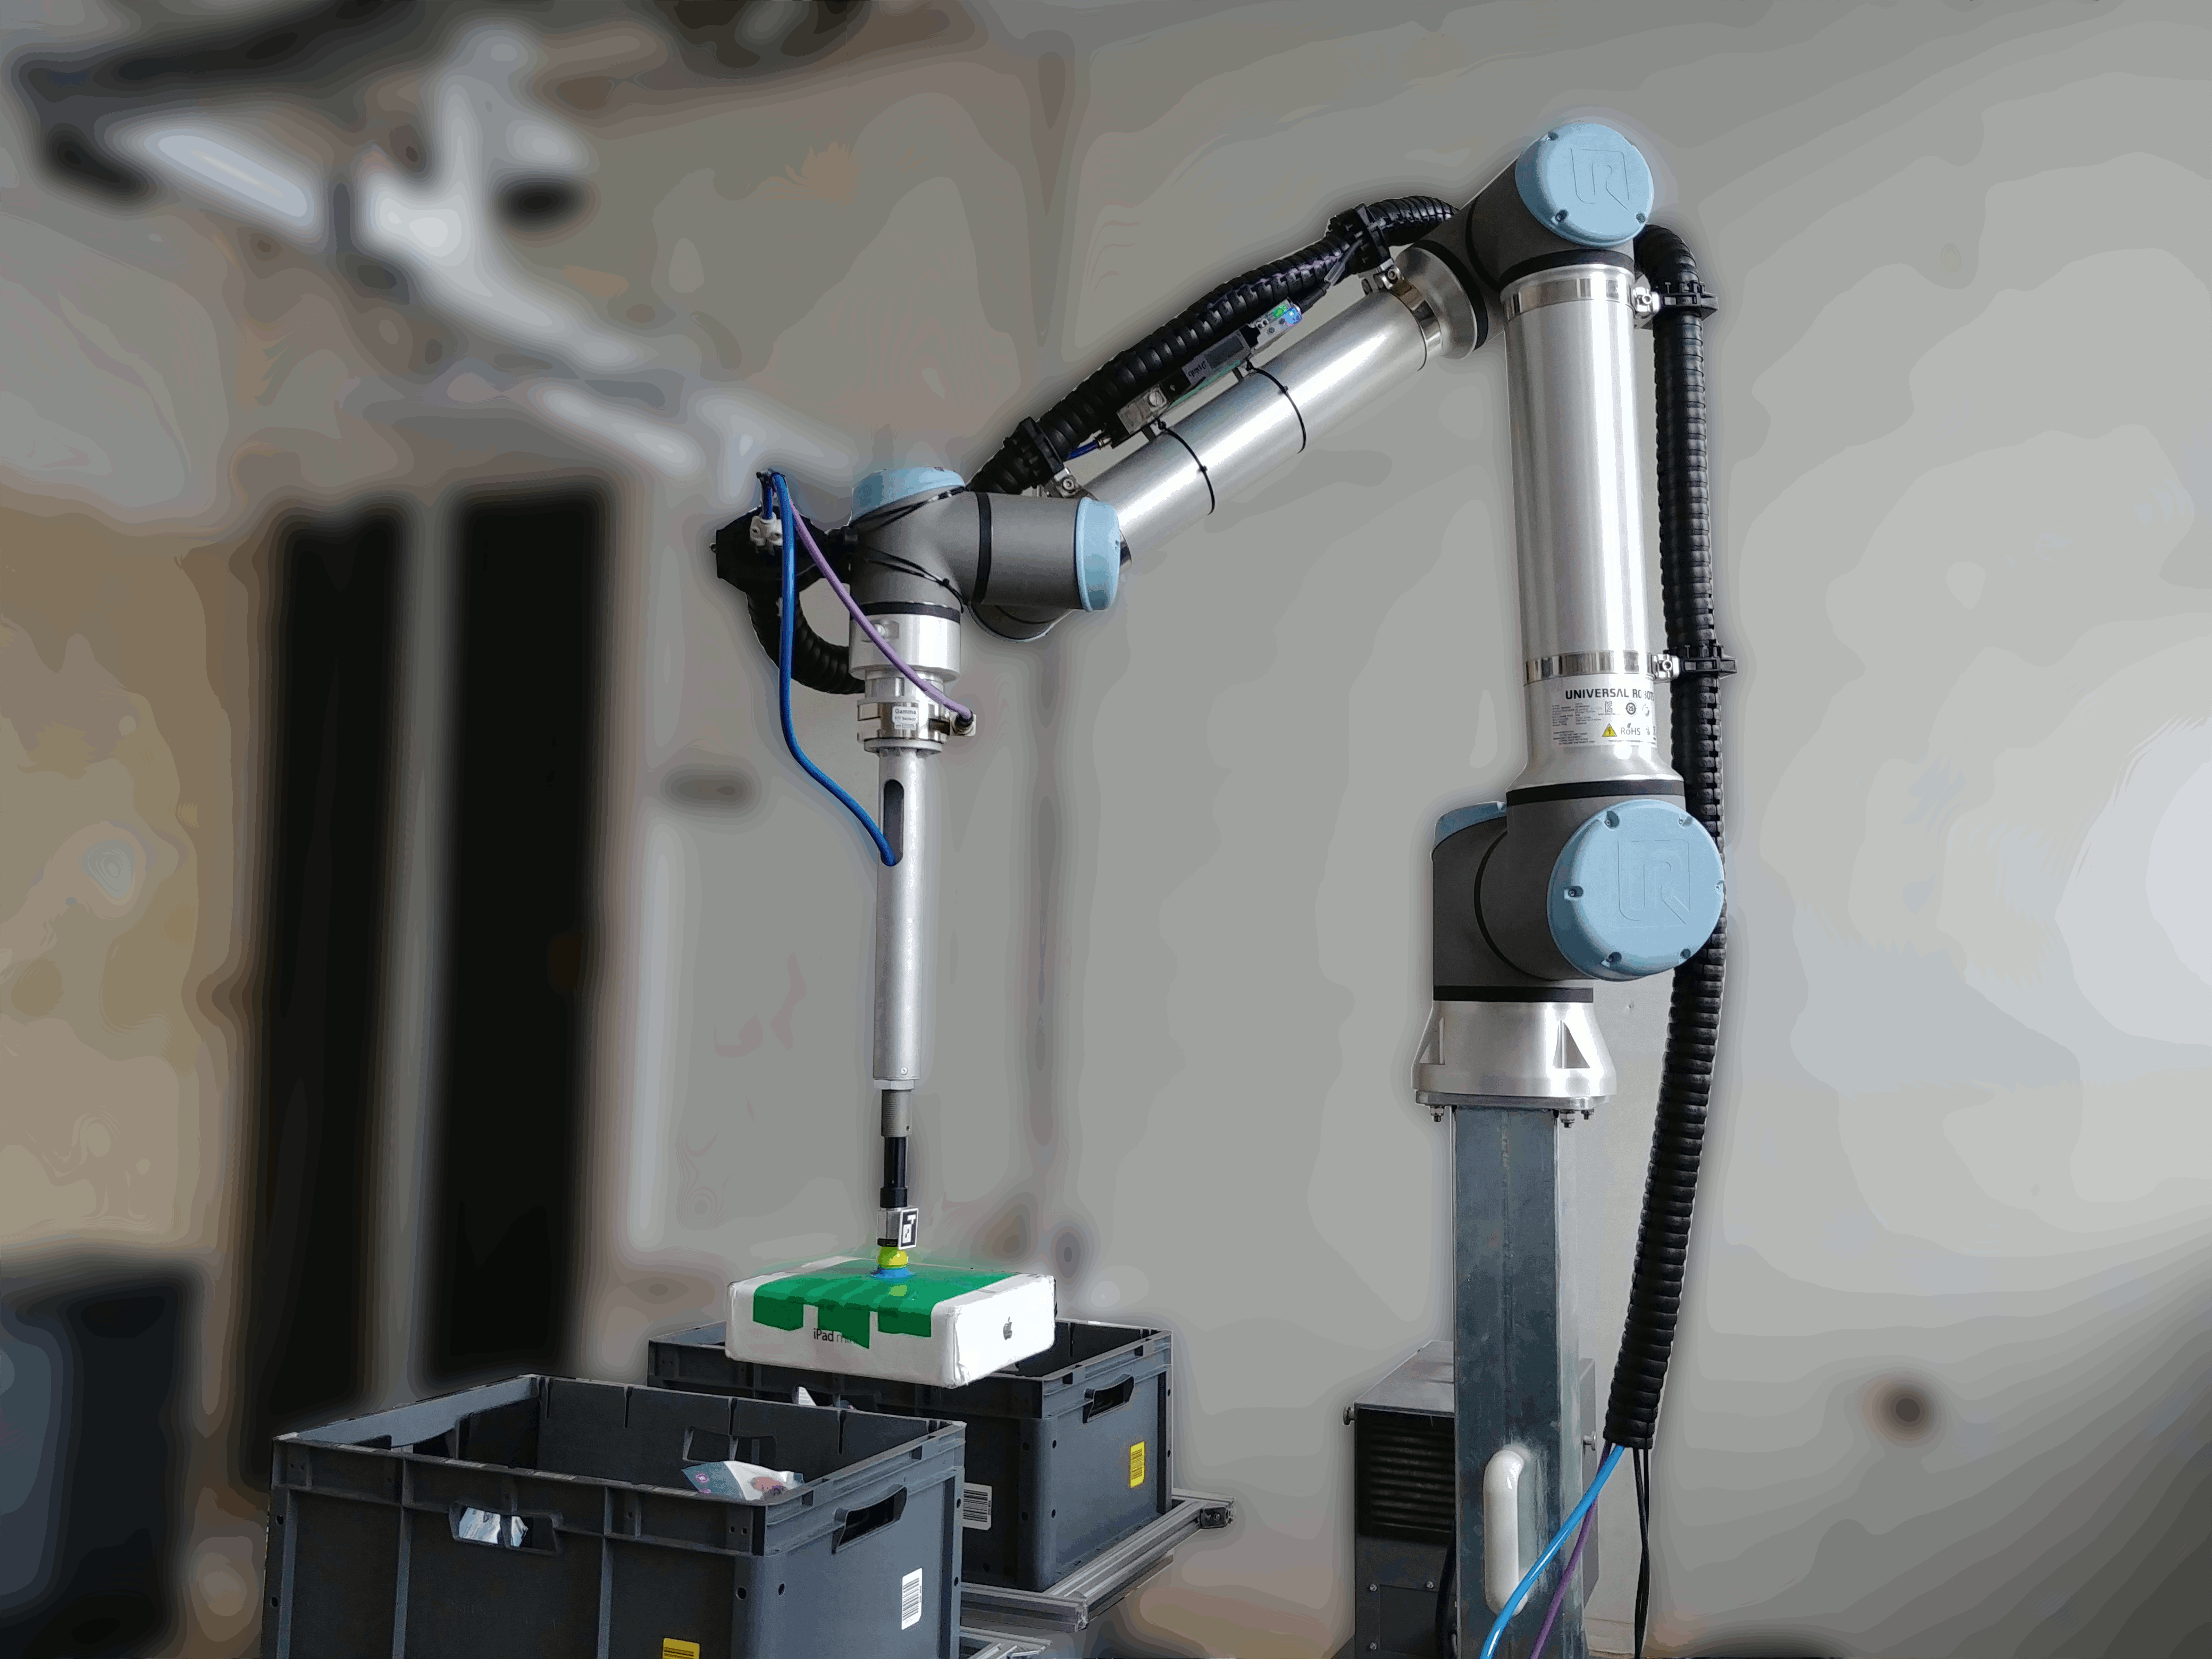
\includegraphics[width=\linewidth]{figs/picture_of_ur_indexed.png}
    \caption{Setup for the RMSD model}
  \end{figure}
\end{column}
\end{columns}

\end{frame}

%------------------------------------------------

\begin{frame}
\frametitle{Results - Rigid model and classical Least-Squares}
\begin{columns}
  \column{37em}
  \begin{figure}
    \centering
    \includegraphics[scale=0.19]{figs/totes_ipad.pdf}
  \end{figure}
\end{columns}
\end{frame}

%------------------------------------------------

\begin{frame}
\frametitle{Results - Rotational Mass Spring Damper and RTLS}
\begin{columns}
  \column{37em}
  \begin{figure}
    \centering
    \includegraphics[scale=0.19]{figs/totes_rtls.pdf}
  \end{figure}
\end{columns}
\end{frame}


%------------------------------------------------
\begin{frame}
\frametitle{Conclusion}
\begin{columns}
\column{37em}
\begin{itemize}\itemsep1em
  \justifying
  \item Rotational Mass Spring Damper model
  \begin{itemize}
    \item \textcolor{TextGreen}{relevant model for the suction cup}
    \item \textcolor{TextGreen}{computation of the orientation of the item}
    \item \textcolor{darkred}{hard to implement online}
  \end{itemize}
  \item RTLS and RMSD approaches improve the performance
  \item Future Work:
  \begin{itemize}
    \item Exciting trajectories for calibration
    \item Recursive General Total Least-Squares with Noise Covoriance Estimation for a better precision and information on the reliability of the estimation
    \item Fully on-line method
  \end{itemize}
\end{itemize}

\end{columns}
\end{frame}

%------------------------------------------------
\begin{frame}
\begin{columns}
\column{37em}
\vspace{1cm}
\Huge{\centerline{\usebeamercolor[fg]{title}Thanks!}}
\end{columns}
\end{frame}

%%%%%%%%%%%%%%%%%%%%%%%%%%%%%%%%%%%%%%%%%
%%%%%%%%%%%% BACK-UP SLIDES %%%%%%%%%%%%%
%%%%%%%%%%%%%%%%%%%%%%%%%%%%%%%%%%%%%%%%%

%------------------------------------------------
\begin{frame}
\frametitle{Filters – Euler's angles continuity and uniqueness filter}
\begin{columns}
\begin{column}{0.5\textwidth}
  \begin{itemize}\itemsep1em
    \justifying
    \item Uniqueness quaternion filter:
    \begin{itemize}
      \item Convert the RPY angles to quaternion
      \item Convert back to RPY angles
    \end{itemize}
    \item Continuity filter \\
    From $[-\pi, \pi]$ to $[-\infty, +\infty]$
  \end{itemize}
\end{column}
\begin{column}{0.5\textwidth}  %%<--- here
  \begin{figure}
    \centering
    \includegraphics[scale=0.12]{figs/maria_orientation_filtered_02.pdf}
    \caption{Raw and filtered RPY angles}
  \end{figure}
\end{column}
\end{columns}

\end{frame}

%------------------------------------------------
\begin{frame}
\frametitle{Filters – Euler's angles continuity and uniqueness filter}
\begin{columns}
  \column{37em}
  \begin{figure}
    \centering
    \includegraphics[scale=0.19]{figs/maria_orientation_filtered_02.pdf}
  \end{figure}
\end{columns}
\end{frame}


%------------------------------------------------
\begin{frame}
\frametitle{Filters – Low pass filter}
Noise in FT sensor measurement. Filter high frequency harmonics.
\begin{columns}
\begin{column}{0.5\textwidth}
  \begin{itemize}\itemsep1em
    \justifying
    \item Low-pass \textsc{Butterworth} filter
    \begin{itemize}
      \item flat frequency response in pass-band
      \item maximally flat magnitude filter
      \item applied twice: forward and backward
    \end{itemize}
  \end{itemize}
\end{column}
\begin{column}{0.5\textwidth}  %%<--- here
  \begin{figure}
    \centering
    \includegraphics[scale=0.12]{figs/maria_torque.pdf}
    \caption{Raw and filtered torque}
  \end{figure}
\end{column}
\end{columns}

\end{frame}

%------------------------------------------------
\begin{frame}
\frametitle{Filters – Euler's angles continuity and uniqueness filter}
\begin{columns}
  \column{37em}
  \begin{figure}
    \centering
    \includegraphics[scale=0.19]{figs/maria_torque.pdf}
  \end{figure}
\end{columns}
\end{frame}

%------------------------------------------------
\begin{frame}
\frametitle{Filters – Smoothing derivated signals}
Noise in TCP pose signal: classical iterative method ineffective
\begin{columns}
\begin{column}{0.5\textwidth}
  \begin{itemize}\itemsep1em
    \justifying
    \item \textsc{Savitzky-Golay} filter
    \begin{itemize}
      \item convolution process with low-degree polynomials on a sub-set
      \item curve fitting with linear Least-Squares
      \item derivation of the polynomials
    \end{itemize}
  \end{itemize}
\end{column}
\begin{column}{0.5\textwidth}  %%<--- here
  \begin{figure}
    \centering
    \includegraphics[scale=0.12]{figs/maria_angular_acceleration.pdf}
    \caption{Classical and filtered TCP angular acceleration}
  \end{figure}
\end{column}
\end{columns}

\end{frame}

%------------------------------------------------
\begin{frame}
\frametitle{Filters – Euler's angles continuity and uniqueness filter}
\begin{columns}
  \column{37em}
  \begin{figure}
    \centering
    \includegraphics[scale=0.19]{figs/maria_angular_acceleration.pdf}
  \end{figure}
\end{columns}
\end{frame}

%------------------------------------------------
\begin{frame}
\frametitle{Calibration of the properties of the system}
\begin{columns}
\column{37em}
\begin{itemize}\itemsep1em
  \justifying
  \item Inertial parameters of the tool
  \begin{itemize}
    \item End-effectors are likely to be unique creations
    \item No ground-truth values provided
    \item Estimation with the rigid model
  \end{itemize}
  \item Spring coefficient and damping coefficient of the suction cup
  \begin{itemize}
    \item As many parameters as there are suction cups
    \item Estimation with the RMSD model and a standard item:
    \begin{itemize}
      \item Mass $m_2$
      \item Center of mass $c_2$
      \item Inertia tensor $I_2$
    \end{itemize}
  \end{itemize}
\end{itemize}
\end{columns}
\end{frame}

%------------------------------------------------
\begin{frame}
\frametitle{Estimation of the inertial parameters of the tool}
\begin{columns}
\column{37em}
  \begin{table}[h]
    \begin{center}
      \renewcommand{\arraystretch}{1.2} % Default value: 1
      \begin{tabular}{l|c|c} % <-- Alignments: 1st column left, 2nd middle and 3rd right, with vertical lines in between
        \textbf{Parameters} & \textbf{Estimated value} & \textbf{Measured value}\\
        \hline
        Mass ($\si{\kilogram}$)  & 0.492 & 0.505 \\
        \hline
        Center of mass $c_x$ ($\si{\meter}$)  & 0.001 & 0.0 \\
        \hline
        Center of mass $c_y$ ($\si{\meter}$)  & 0.0003 & 0.0 \\
        \hline
        Center of mass $c_y$ ($\si{\meter}$)  & 0.181 & 0.19 \\
        \hline
        Inertia $I_{xx}$ ($\si{\kilogram\meter\squared}$)  & $8.7 \times 10^{-4}$ & $5.8 \times 10^{-4}$ \\
        \hline
        Inertia $I_{xy}$ ($\si{\kilogram\meter\squared}$)  & $2.3 \times 10^{-5}$ & 0.0 \\
        \hline
        Inertia $I_{xz}$ ($\si{\kilogram\meter\squared}$)  & $1.8 \times 10^{-5}$ & 0.0 \\
        \hline
        Inertia $I_{yy}$ ($\si{\kilogram\meter\squared}$)  & $5.3 \times 10^{-4}$ & $5.8 \times 10^{-4}$ \\
        \hline
        Inertia $I_{yz}$ ($\si{\kilogram\meter\squared}$)  & $1.1 \times 10^{-5}$ & 0.0 \\
        \hline
        Inertia $I_{zz}$ ($\si{\kilogram\meter\squared}$)  & 0.0017 & 0.001 \\
        \hline
      \end{tabular}
    \end{center}
    \vspace*{-0.1cm}
    \caption{Comparison between the estimated and measured inertial parameters of the tool.\label{tab:results:calibration-tool}}
  \end{table}
\end{columns}

\end{frame}

%------------------------------------------------
\begin{frame}
\frametitle{Estimation of the suction cup parameters}
\begin{columns}
  \column{37em}
  \begin{figure}
    \centering
    \includegraphics[scale=0.25]{figs/calib_torque_y.pdf}
    \vspace*{-0.3cm}
    \caption{Torque acting on the tool about the $y$-axis}
  \end{figure}
\end{columns}
\end{frame}

%------------------------------------------------
\begin{frame}
\frametitle{Estimation of the suction cup parameters}
\begin{columns}
  \column{37em}
  \begin{figure}
    \centering
    \includegraphics[scale=0.3]{figs/angle_y.pdf}
    \vspace*{-0.7cm}
    \caption{Orientation of the load about the $y$-axis}
  \end{figure}
\end{columns}
\end{frame}

%------------------------------------------------
\begin{frame}
\frametitle{Results - Rigid model and classical Least-Squares}
\begin{columns}
  \column{37em}
  \begin{figure}
    \centering
    \includegraphics[scale=0.19]{figs/all_sku.pdf}
  \end{figure}
\end{columns}
\end{frame}


\end{document}
% darkred TextGreen Ocean
